\chapter{Achievements}
\par I tried to apply agile methods during the development of the application. I split each part in daily tasks and I reported it the day after if they were not done. When I spent more than three days on a single task I informed Pierluigi and I looked for help in the lab. It worked really well and I can tell know that if works even on a project where I was single. This method matched with my rhythm and my progression.
\par In the figure \ref{gantt} we can see all the progression of the internship (all the tasks are explained in the following pages). I set two important meetings for the project, but there were meetings with Mario Vento for global satisfaction and progression feedbacks that I did not mention. Globally, I think my time was well organized and I had a regular progression.

	\begin{figure}[h]
		\begin{center}
			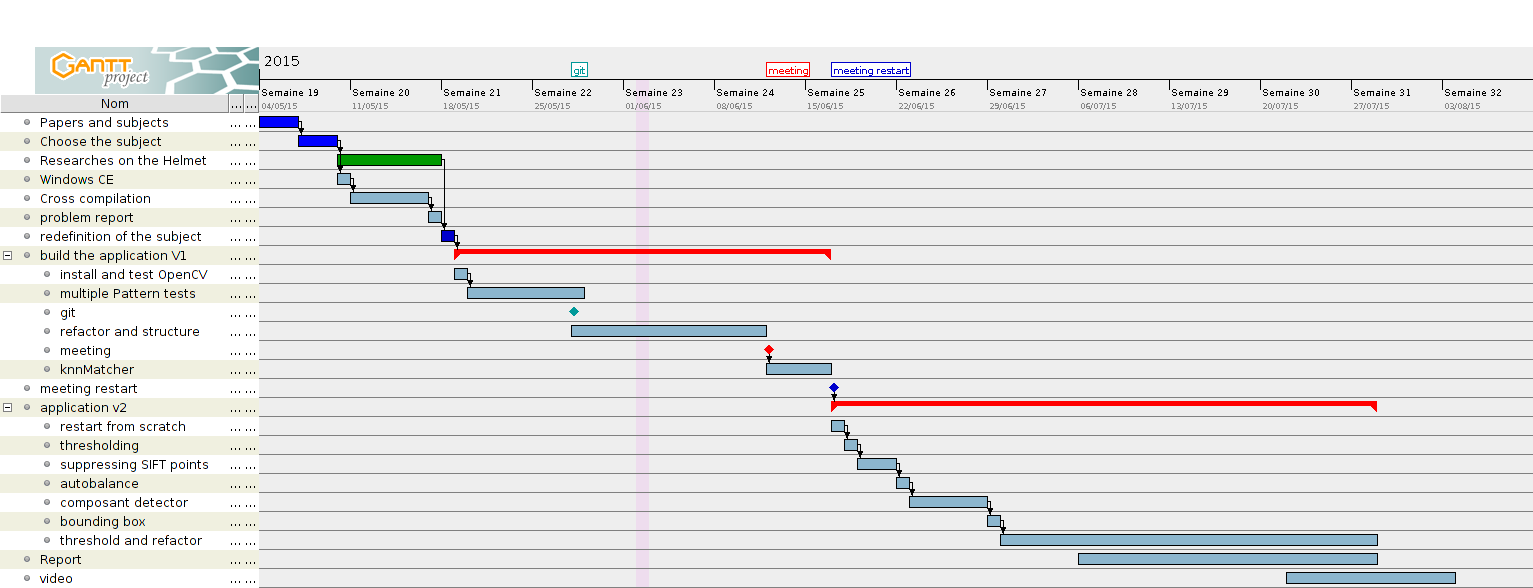
\includegraphics[width=16cm]{images_not_compressed/gantt.png}
			\caption{Gantt chart}
			\label{gantt}	
		\end{center}
	\end{figure}
	
	
	\section{Installation and tests}
	

\par For keeping the idea of two distinct projects, this part will turn around on issues and successes. I will explain how I corrected them if I could. I will gather the installations for OpenCV and the cross toolchain because the main idea is the same. Then I will divide the technical part in two as usual.


	\subsection{Helmet}
	\subsubsection{Cross GCC}
	
	\par Cross GCC is pretty easy to install, you have to get the archeve and compile the cross compiler for your architecture. First of all I saw in that the tutorial required an Ubuntu 12.10LTS\footnote{Long Lime Support of Linux based operating system.} at least. I used virtual box to get a virtual machin\footnote{Software to emulate operating systems} of this distribution on my windows operating system. Next, I simply followed the tutorial that explains how to install the cross compiler. This part was really easy, after have downloaded GNU cross G++ I ran the commands and the compiler was installed.
	
	\subsubsection{Kernel compilation}
	
	\par The compilation of the kernel is almost the same as the compiler, except that you compile for another platform \footnote{Here it is the OMAP3.}. Of course the compiler handles ARM cortex A8 for TI OMAP3. I just had to check the option for this CPU\footnote{Central processing unit.} during the installation and then the kernel I compiled was compatible with this architecture. As a result, I got a file system\footnote{Set of files, which represent the distribution of Linux I chose (Debian)}  ready to boot on an ARM device.
	
	
	\subsubsection{Tests}
	
	\par Once the file system is compiled, I had to put it inside the helmet memory. Two main problems remained, first the helmet memory was inside the helmet itself and not in the memory stick. And secondly, you can only copy files using Windows CE on the intern memory. This means that you cannot erase Windows CE file system and replace it by another.
	\par That is where I found out that the project was compromised. I had few knowledges in Windows CE\footnote{Light operating system developed by Microsoft} and the fact the helmet was not started in the first place meant that I had to repair this Windows CE first. Moreover the interface is voice commanded. I estimated the time to solve the problem longer than my internship.
	\par Thus, I tried to launch the file system on qEmu which failed. When I explained all of that to my superior they decided to change the project. Still, I had to send a little report to Mario Vento with the different problems that I encountered during the project.
	
	\subsection{Pattern scanner}
	\subsubsection{OpenCV installation}

	\par I installed OpenCV 3.0 which is the last version and tried it. It has a base for basic image applications and modules that you can install by adding them to the module folder and compile them. Unfortunately, one module required to perform the test was not working with the 3.0 version. It is the non free module. I tried several times, but I finally decided to switch back to a previous version. After uninstall everything and install the 2.4.9 version. The module was functional. I tried the code of the tutorial ~\hyperlink{opencv}{I quote earlier} and I had the first pattern recognition result. That took me 4 days in total including the eclipse configuration that require adding all the libraries in the configuration of the compiler one by one.
	
	\section{Main problems}	
	\subsection{Related to the helmet}
	\par I had several issues before I began working on the helmet. Some of them are related to the hardware and others to the operating system.
	\subsubsection{Hardware}
	\par The first problem we encountered was getting the component references of the helmet like processor, camera, mother board, etc. Pierluigi, my tutor sent mails to the company which proposed the project. Unfortunately, they were not able to gain access to this information. I looked for it on the manuals and documentation that Pierluigi gave to me and the Internet. Every time, I could not get the precise references, only the names of the product are available.

	\par Besides, there was little issues with the helmet itself because the alimentation module was missing. That module allows us to plug the helmet directly to the outlet. To resolve the problem I had to load the batteries and plug it to the helmet to boot\footnote{Start the operating system.} it.

	\subsubsection{Emulator}
	
	\par I downloaded and easily install the emulator (qEmul) advised in the tutorial that I followed but I couldn't run the operating system on it. The operating system started with a black screen and then nothing happened. I did not find a solution to this problem because I found out that the project was already compromised by the fact that we did not have access to the references of the components. Still, I was a little bit surprised that the emulation was not working because all the steps of the tutorial was working except this one.
	
	\subsubsection{The operating system}
	
	\par Window CE 6.0 was made for embedded systems to concurrence Linux. The problem with the helmet was the fact that the system could only be updated and not erased. For example, if somebody wants to replace the file system, he has to put on an SD card, an update of windows that is compatible. This update would be written on the intern memory to replace the actual system. Unfortunately, except Microsoft I do not know if somebody can do this which means that Linux will not work. Perhaps there are other ways to do it, but I do not have that kind of skills. I looked for forum on the Internet, but Windows CE does not have a real community.
	
	\subsection{Related to the software}
	
	\subsubsection{The matcher}
	
	\par After 3 days, making some tests and learn about the matching system. Alessia, the thesis companion of Mario Vento made me realize that I was on the wrong way using the match function of OpenCV. In fact, I could not find multiple patterns with that method because it selects the nearest descriptors\footnote{Those which have a minimum hamming distance likeness}. The result was that I had to launch several times the algorithm to get new matches again and again. I found the knnmatcher that perform a full matching and keeps the N best matches. That was not enough so I switched to the radius matcher that need a threshold parameter. That is finally how I introduce the threshold in the program. This value depends on the object, the distance and the conditions of the scene. In another way, the matcher keeps the matches which differ less than the threshold.
	\par The algorithm returns a vector\footnote{Collection of the standard library in C++.} of vector of DMatches\footnote{A structure representing each match.} so I put it in a simple vector of DMatches and it gave me very good results. The algorithm was able to find multiple times the same match on the scene. In the figure \ref{matches} we can see the fact that every time the pattern is represented it has matched it. Not just the best ones which here corresponds to the first one on the left.
	
	
	\begin{figure}[h]
		\begin{center}
			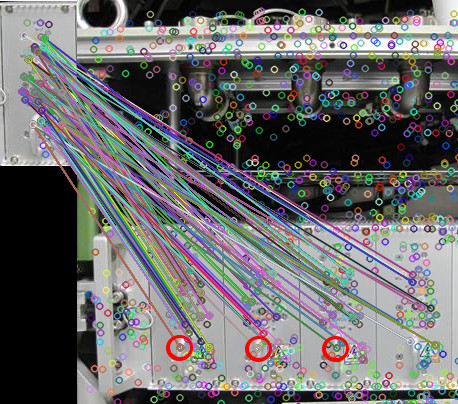
\includegraphics[width=10cm]{images_not_compressed/matches.jpg}
			\caption{Simple draw of radius match with 3 times the same match surroundded in red}
			\label{matches}	
		\end{center}
	\end{figure}
	
	\subsubsection[Multiple pattern]{Get many time the same pattern}

	\par With Pierluigi, we agreed on two methods. The easy one was to draw in black the image and then make the homography another time. The hardest one was to look for the key points and descriptor inside the corners\footnote{Those we just found.} and erase them of their containers. Then do the homography again to get another pattern. I began with the second one that sounded more relevant. 
	
	\par To be clear, I have to present the DMatch structure that is detailed in the \hyperlink{structDMatch}{annexes}\ref{struct}. The important attributes are the train index and the query index. They represent the fact that a descriptor has been found in the two images. But only the index of the descriptor is stored.
	
	\par I first thought I could easily get the points that gave me the corners after the homography. In fact, I needed to remove the points that concern the pattern that has been recognized by the homography. There was no other way but to extract all the indexes of the points inside the corners I just found and remove them from the vectors. By chance, the homography takes in parameter vectors of points describing the positions of the descriptors (and the key points by the same way). 
	\par On the first version of this algorithm I was looking if the point was in the bounds represented by the 4 segments of the rectangle of the pattern found. I found out when I was rotating the image that the points was removed the wrong way because the shape of the pattern was a diamond. A lot of points were considered out of the bounds and the other that had nothing to do with the pattern were removed.
	\par I found on the internet, a method~\cite{InOut} that provides the answer of my problem in O(n)\footnote{Complexity of the algorithm here n represents the number of points in the container.}. This method finds the number of edges that a line from one of the points to the infinite crosses. If it is odd then the point is inside the polygon, otherwise it is outside. The picture~\ref{OutIn} illustrate the idea.
	\begin{figure}[h]
		\begin{center}
			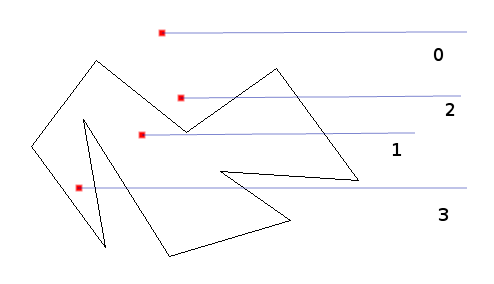
\includegraphics[width=10cm]{images_not_compressed/isIn.png}
			\caption{Illustration of the algorithm which tell if a point is inside a polygon}
			\label{OutIn}	
		\end{center}
	\end{figure}
	\subsubsection{Corners}
	\par OpenCV does not implement a structure for the corners. The corners correspond to the vertices of the polygon that represents the pattern. I isolated them in a structure because that was a good proof of the fact that the algorithm found efficiently a pattern. It also helped me to find out that the first version of the algorithm which removes the points was malfunctioning.
	\par I let the structure as it is because I told myself that, in the future, the application could need the corners of the pattern to compute move analysis for example. 	
	
	\subsubsection{Others}
	
	\par My biggest parallel achievement is an algorithm that helps the user of the application to find the best threshold for his patterns. It depends on the number of patterns you want to recognize because the threshold must be higher for certain conditions and, more there is a pattern in the image, the more there are different conditions. 
	\par The algorithm takes a scene and a pattern in input plus the number of times the pattern is represented in the image. The result of the algorithm is the first threshold that got all the patterns in the image. It computes a range of 150 values, that is why I can take several seconds to compute.
	
	\begin{figure}[h]
		\begin{center}
			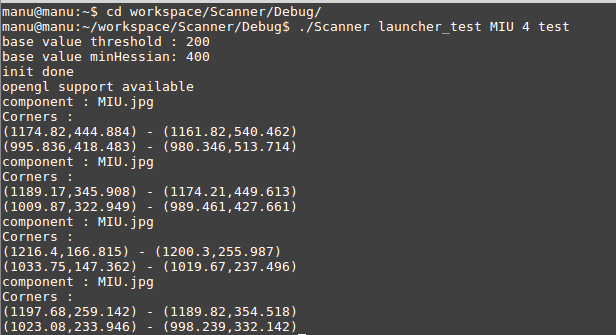
\includegraphics[width=10cm]{images_not_compressed/tester.png}
			\caption{Screenshot of the algorithm finding four times the MI unit pattern}
		\end{center}
	\end{figure}	
	
	\par We can see here that for units has been found with the positions of their corners.
	
	\par I also had to create a video for Pierluigi to showcase the possibilities of my application. Therefore, I used VLC media player to stream my screen during a demonstration. I turned the stream into mp4 and used Kdenliv to make some modification and add titles. When the result was good enough, I used GNOME Subtitles to write a .str\footnote{.str is the standard format of subtitle files.} file that corresponded to the video. Then I uploaded the video on Youtube to share it with Pierluigi. I made some changes in the beginning of the video several times. That took me a long time because I had to change manually all the subtitles that passes after the added or suppressed section.
	\par The video is accessible here : \url{https://youtu.be/q23RjtwAqDU} you can see in the figure the page where I edited the properties and added the subtitles to make it available on Youtube.
